\section{Basic parallel algorithms \& patterns}
\subsection{Reduce}
Consider the situation, when we need to add all the array's elements together. In \verb|C++|, one could use 
the STL algorithm \verb|accumulate()| function. In a more primitive implementation, we would do a single for-loop 
and accumulate the results in one variable. The complexity of such an algorithm would then be about $O(n)$, where 
$n$ - the length of the array. However, one could add some parallelism to this algorithm. 
Indeed, at first iteration, what we would 
do is to add the 0th element with the 1st, the 2nd with the 3rd, the 4th with the 5th, etc... Notice that 
all of these $\nicefrac{N}{2}$ additions additions can be done in parallel (that is, each thread does one addition). The next \textit{iteration}, would be 
summing the result of the sum of 0th and 1st with the sum of 2nd and 3rd, thus giving a total of 
$\nicefrac{N}{4}$ additions (instead of $\nicefrac{N}{2}$ ) . 
Therefore, the number of necessary divisions on the next step, will be the half of those, during the previous ones.
As those divisions are performed in parallel, this algorithm looks like a log-scale complexity. 

\begin{figure}
   \centering
   \begin{subfigure}[t]{0.45\textwidth}
        \centering
        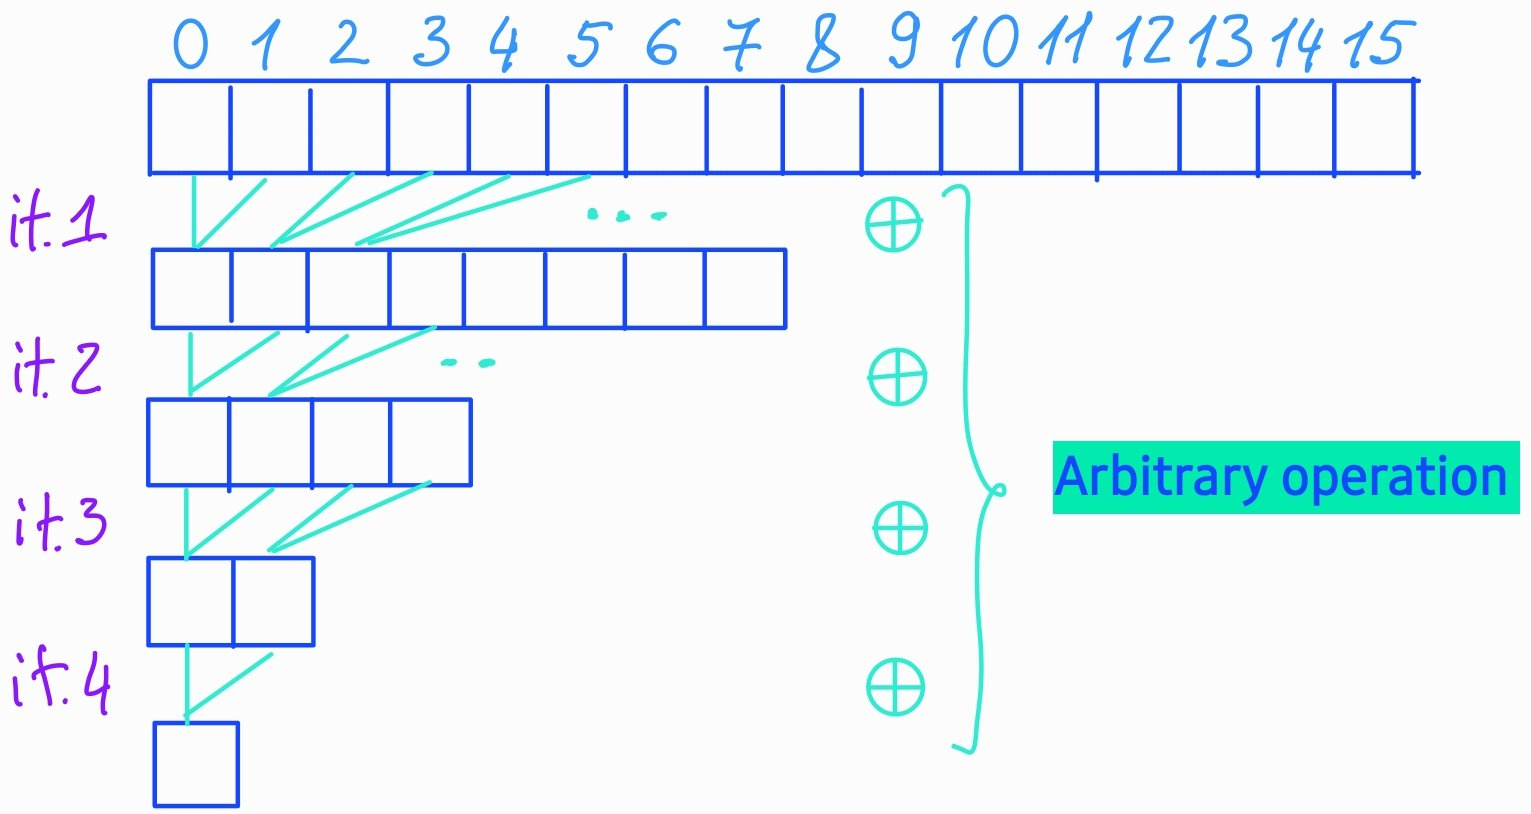
\includegraphics[width=6cm]{pngs/reduce_global.jpg}
        \label{fig:static}
    \end{subfigure}
    \begin{subfigure}[t]{0.45\textwidth}
        \centering
        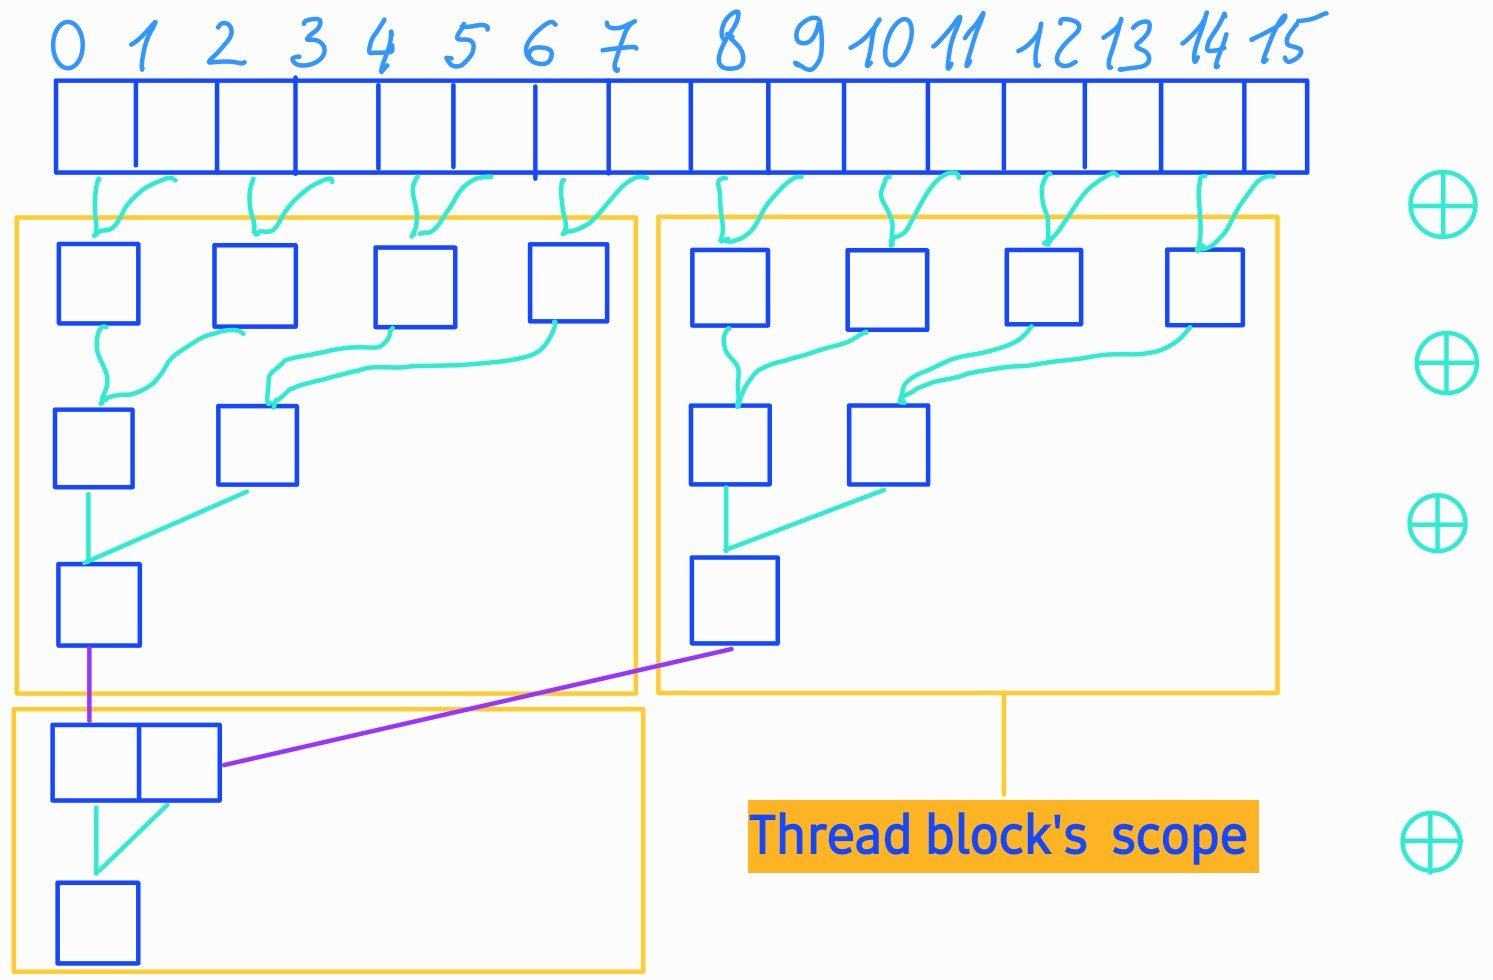
\includegraphics[width=6cm]{pngs/reduce_shared.jpg}
        \label{fig:dynamic}
    \end{subfigure}
\label{fig:reduce}
    \caption{Reduce algorithm with differnet strategies.}
\end{figure}

\subsubsection*{Global memory reduce}
Let's first have a look at a \sout{not so} naive implementation of the discussed reduce algorithm on the GPU.
Once again, we're looking at a simplified version of the code, without implementing memory allocation, copy, etc... 
(note that in this case, we use simple global mamory with \verb|cudaMalloc()|). The implementation of this is given by \autoref{listing:global_reduction}.


\begin{listing}
\begin{minted}[frame=single, framesep=1mm]{cuda}
__global__ void reduce_global_kernel(float *data_out,\
               float *data_in, int stride, int size) {
int idx_x = blockIdx.x * blockDim.x + threadIdx.x;
if(idx_x + stride < size){
data_out[idx_x] += data_in[idx_x + stride];
}
}

void reduce_global(float *d_out, float *d_in, int n_threads, int size) {
int n_blocks = (size + n_threads - 1) / n_threads;
for (int stride = 1; stride < size; stride *= 2){
   reduce_global_kernel<<<n_blocks, n_threads>>>(d_out, d_in, stride, size);
}
}

//main()
\end{minted}
    \caption{Global memory reduction. \cite{tuomanen2018hands}}
    \label{listing:global_reduction}
\end{listing}

\begin{wrapfigure}{R}{0.45\textwidth}
   \vspace{-0.9cm}
   \begin{center}
   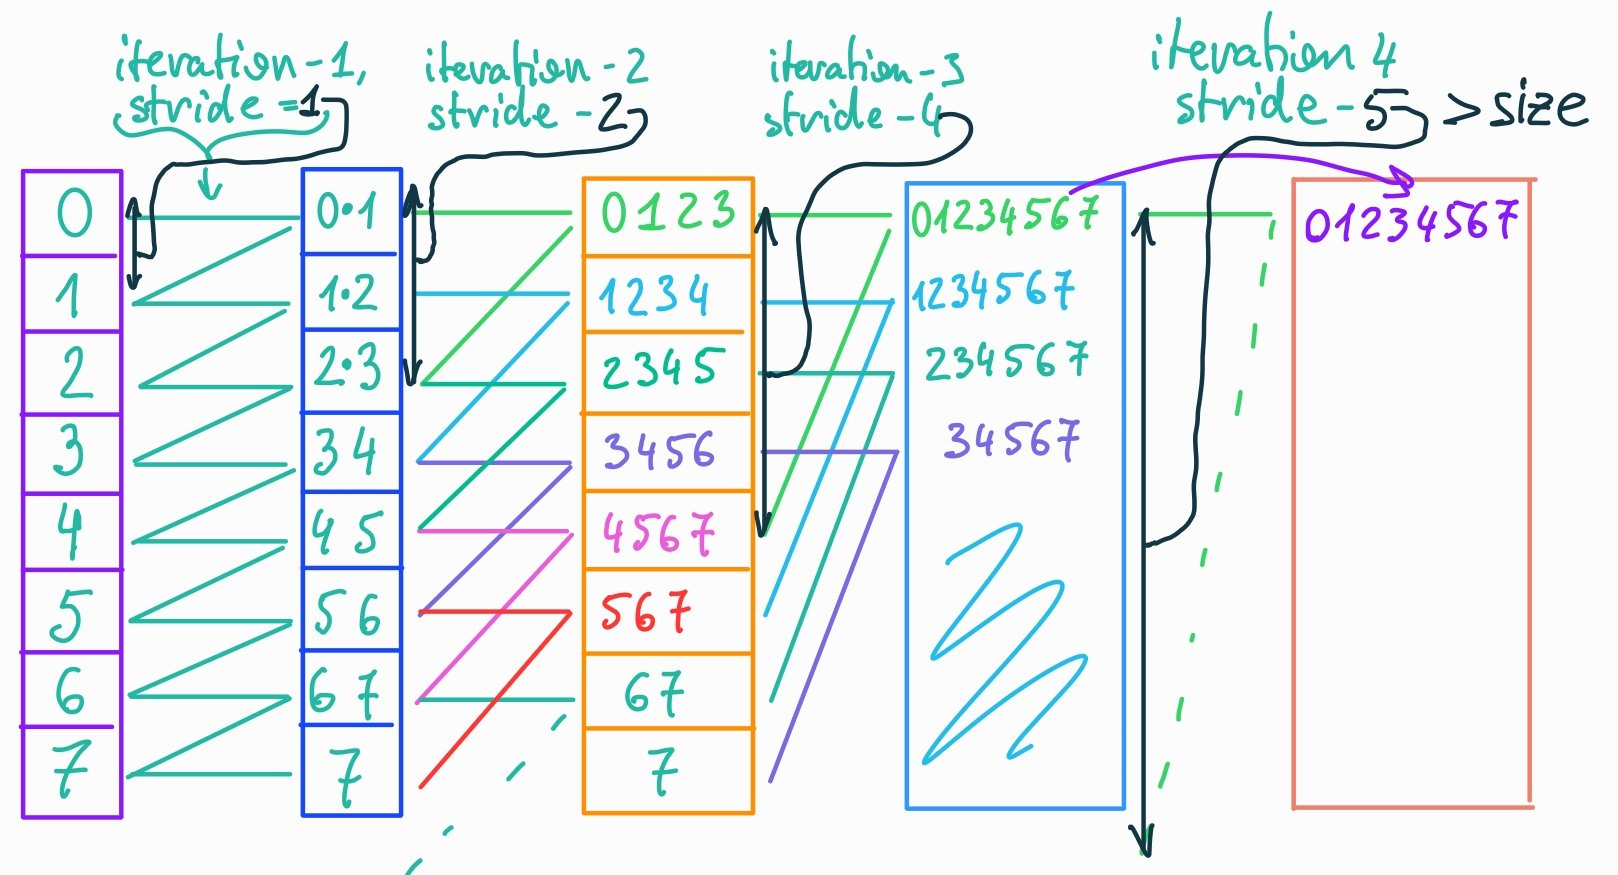
\includegraphics[width=0.45\textwidth]{pngs/reduce_only_global.jpg}
   \end{center}
   \vspace{-0.5cm}
   \captionsetup{justification=raggedleft}
   \caption{The description of every iteration, for the global memory 
   reuction kernel. Note the how stride is doubling every iteration, 
   ,and how the elements are accumulating in the very first (0th) element of the output data. 
   One should understand, that the code works for arbitrary number of blocks, as we're working with global 
   memory, visible to all threads in all blocks}
   \label{fig:reduced_global_only}
\end{wrapfigure}

Okay, let's discuss the \autoref{listing:global_reduction}. First in the host function, we define the number of blocks. 
In this case, this number is not so important. It would be important to optimize the execution, 
by taking into account the notion of warps, etc... The important part is the loop in the host code and 
the device kernel. We will try to do the debugger's job and inspect the steps. 
During the first iteration, the value of \verb|stride| is 1. The important point is that the thread id, 
computed in the kernel does not depend on the value of the stride. This is because we're working with the global 
memory, and the access is global.

Suppose the size is $32$, partitioned into 1 block. Then for the first iteration, we'll get, 
\verb|out[0] = [0]+[1]|, \verb|out[1] = [1]+[2]|, ... \verb|out[30] = [30] + [31]|. This is exactly the first iteration, 
showed in \autoref{fig:reduced_global_only} (the case of size=8). Then, during the next iteration, we're 
\textit{jumping} over 2 next elements, and adding them, in order to get the sum of $N_{stride}$ elements, and save them 
into the \verb|data_out[0]|. Let me mention, that this process is illustrated in the image above \autoref{fig:reduced_global_only}.

This algorithm is, maybe, not easy to understand, but is very fundamental parallel algorithm. Both the algorithm, and the 
way of analyzing the problem. However, it can be optimized using the block's shared memory.


\begin{wrapfigure}{R}{0.5\textwidth}
   \vspace{-0.9cm}
   \begin{center}
   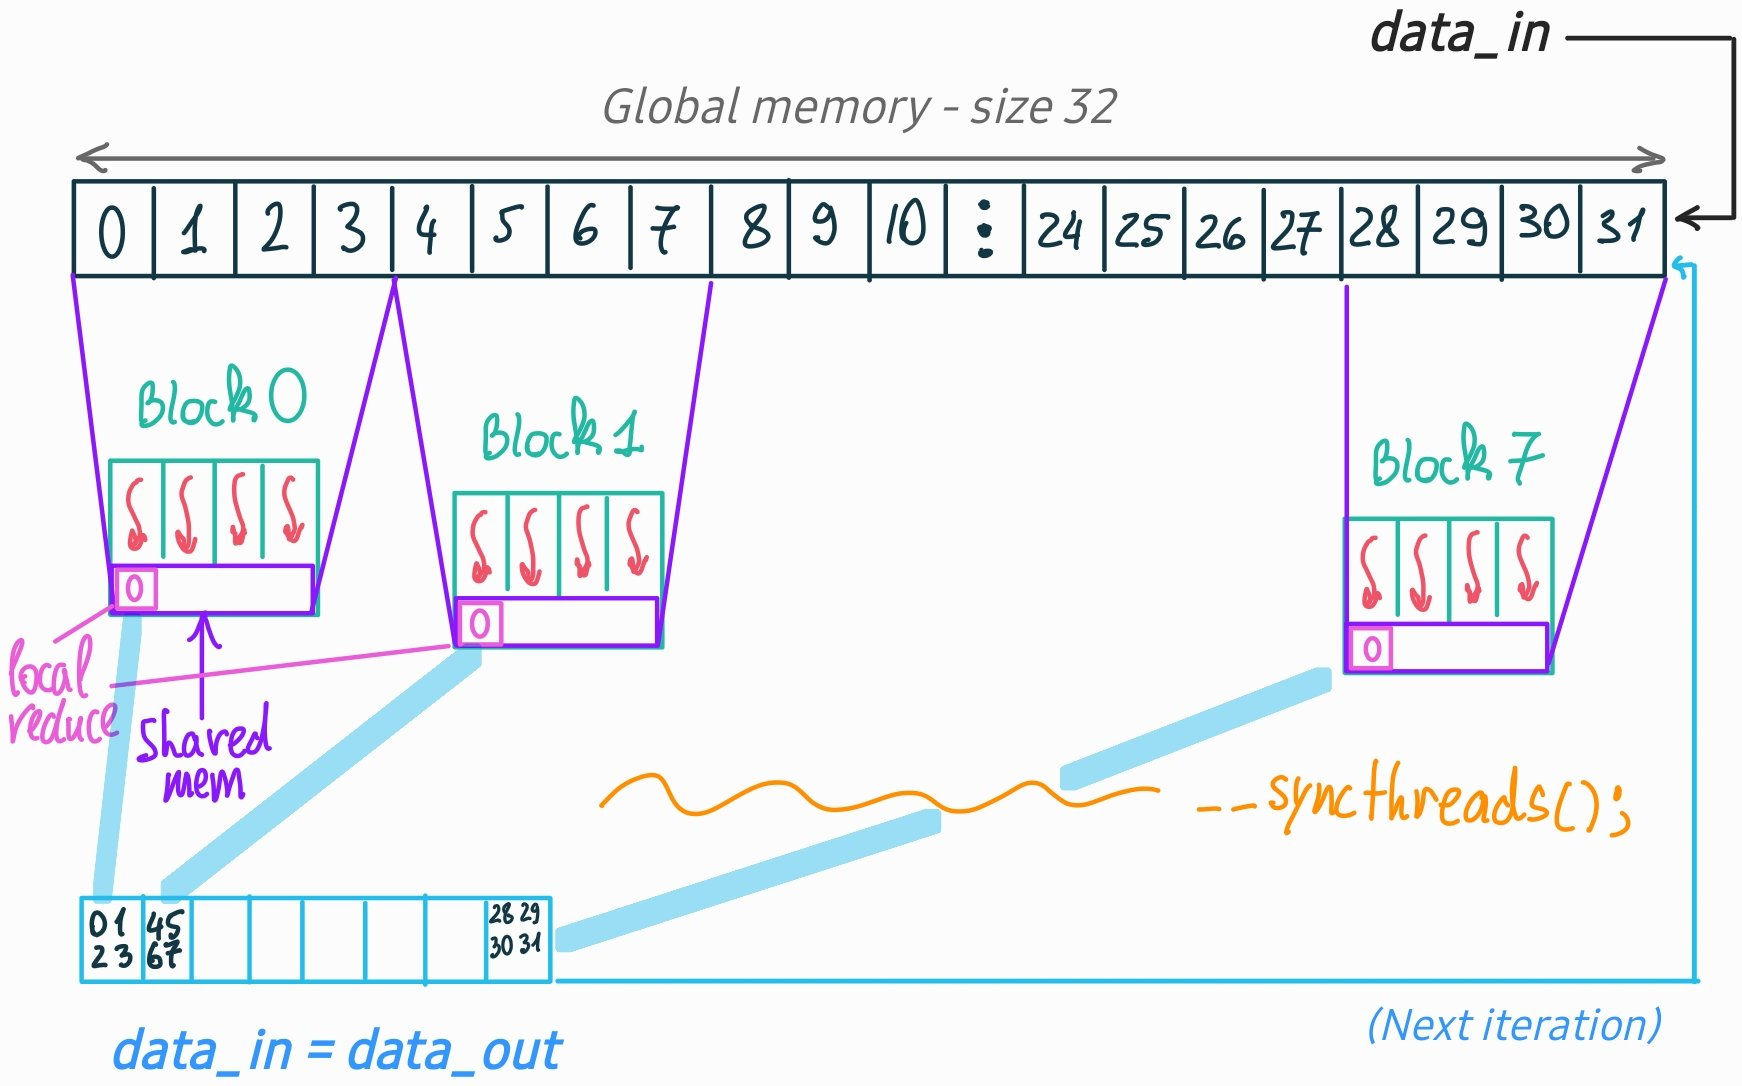
\includegraphics[width=0.5\textwidth]{pngs/shared_reduce.jpg}
   \end{center}
   \vspace{-0.5cm}
   \captionsetup{justification=raggedleft}
   \caption{Reduce algorithm using shared memory.}
   \label{fig:shared_reduce}
\end{wrapfigure}



\subsubsection*{Shared memory reduce}
As we've discussed several times above, the shared memory access has low latency. The idea is thus 
to do a local copy of the data to each block. As the shared memory's size is limited, we \textbf{map} the 
data pieces to each block (see figure).

Now, let's try to understand it together in more detail, using well-defined numbers of threads and blocks, 
to make things more illustrative. Trying to keep in mind both the illustration (\autoref{fig:shared_reduce}).

\begin{listing}
\inputminted[frame=single, framesep=1mm, linenos=true]{cuda}{cucodes/shared_rreduced.cu}
\caption{Optimized reduce, with shared memory. \cite{tuomanen2018hands}}
\end{listing}

We omit the \verb|main()| function and the host/device memory allocation/copy.
Line $2$ declares the function, which will be calling the kernel. Line $3$ copies memory 
\verb|cudaMemcpyDeviceToDevice|. This is done in order to make sure we're working with the same memory locally allocated on the device.
This is illustrated with the bottom blue arrow. 
\paragraph*{First iteration}
For the first iteration, we're associating the variable \verb|int size| to be the litteral 
number of elements to be reduced. In our case, it is $32$. The next declared variable \verb|int n_bl| is, 
as the name suggests, the size of the block. As we're working with the shared memory, each shared memory 
will be allocated for one specific block, as shown in figure. In our case, we've chosen \textit{nice} 
numbers, so that \verb|n_thr * n_bl = size = 32|, with \verb|n_thr| - the number of threads per each block.
On line $6$, we're finally invoking the kernel with the initial $8\times 4$ dimensions (the first 2 parameters in the angle brackets). 
The 3rd parameter in the angle brackets is the size of shared memory, that will be assigned to each block. 
We see this syntax for the first time. This is how we allocate the \textbf{dynamic shared memory}, which we will 
discuss a bit later, as well as the last parameter $0$ (ignore that too for the moment).
For now, this is just shared memory allocation, outside the kernel itself. So we've allocated 
$n_{threads}\times size_{float}$ - the exact amount of shared memory, that will be accessed by the 4 threads. 

Let's move to the kernel body itself. First, on line $12$, our usual procedure, we're assigning a personal 
ID to each thread. Line $13$ declares shared memory with size of $n_{threads}\times size_{float}$, specified outside, 
at the kernel call. This is the dynamic allocation of shared memory with \verb|extern| keyword 
(as said, we'll discuss it later). On Line $14$, we're copying the data to shared memory. Remember, 
the size of shared memory is the size of threads in the block (line $6$). Thus the operation 
SH\_DATA[LOCAL\_THR\_ID] is performed. Line $6$ operation is illustrated with the violet lines - the
mapping between the global to shared memory ($[0:3]_{global}\mapsto [0:3]_{block=0},\text{ } [4:7]_{global}\mapsto [0:3]_{block=1}, \text{...} $).
After copying, we are making sure that \textbf{all} the threads are done copying with \verb|__syncthreads()|. Without that, some problems can occur 
(e.g.if we're starting reducing in 0'th block \textbf{before} all the threads within this blocks are done copying its data).

On line 17, we're starting to perform reduction. Let's first try to ignore the \verb|if| 
condition on line $20$, in order to better understand, why is it, and should be here. The 
dummy variable \verb|stride| varies from 1 to the size of the block -
$1\to 2\to 4\to 8\to 16 \to ...$ (in our case till $8$).% Thus for each thread in the block, 
For example, for a local thread with local ID = $0$, the sum of SH\_MEM[0], SH\_MEM[1], SH\_MEM[2] will be accumulated 
within the loop. For thread with local ID = $1$, the sum of SH\_MEM[1], SH\_MEM[2], SH\_MEM[3] will be accumulated. For
thread with local ID = $2$, the sum of SH\_MEM[2], SH\_MEM[3], SH\_MEM[4], will be accumulated, and so on. 
We have now several problems, e.g. the access to SH\_MEM[4], which is out of bounds, as the size of it is the 
save as number of threads ($4$ in our case). 

Consider now the loop on the global scale/scope, as on line $20$, 
we're checking the global thread ID. Then which threads will access the line $21$, for the dummy variable \verb|stride| = $1$? 
These are threads with global ID $0,2,4,6,8,10,12,14,16, ... $, which corresponds to local threads
$\{0,2\}_{block=0},\text{ }\{0,2\}_{block=1}, ...$ (see violet lines \autoref{fig:shared_reduce}). 
On next iteration of the dummy variable \verb|stride| = $2$, only threads with global 
ID's $0,4,8,12,16$ will access the line $21$, which corresponds to local threads $\{0\}_{block=0},\text{ }\{0\}_{block=1}, ...$

Now, taking into account the two aspects, we can say, that for the first iteration of the dummy variable \verb|stride|=1, the 
the threads with local ID's $0,2$, will accumulate SH\_MEM[0], SH\_MEM[1] \underline{into} 
SH\_MEM[0] and SH\_MEM[2], SH\_MEM[3] \underline{into} SH\_MEM[2] respectively. 
For the next iteration of the dummy variable \verb|stride|=$2$, only the thread with local ID's $0$ 
will accumulate SH\_MEM[0] and SH\_MEM[2] into SH\_MEM[0]. \textbf{But remember: } in the previous iteration, 
the sum of SH\_MEM[0], SH\_MEM[1] was stored in SH\_MEM[0] \textbf{and} SH\_MEM[2], SH\_MEM[3] into SH\_MEM[2]. 
Thus, during the last iteration, we've performed the reducing operation within the block and accumulated the sum into SH\_MEM[0]. 
The line $25$ will simply write the value of SH\_MEM[0] to the output, global memory.  The kernel is done. 

\paragraph*{Next iterations} operate the same way as the first. The only thing that is changing is the number 
of blocks, that the GPU will operate with. This does neither change the workflow, nor even the size of 
shared memory within each block. 

It is quite hard \sout{even maybe very hard} to understand the pipeline of the method execution. 
We should re-read the text above again and again, and try to associate it with the \autoref{fig:shared_reduce}.
To recap the reduce process with shared memory:  

 \begin{itemize}
   \setlength\itemsep{-0.5em}
    \item Define the initial number of threads and blocks, such that they cover the whole 
    array to be reduced (note that \#threads - number of elements on which the reduction will be performed locally).
    \item At every iteration, launch the kernel with the \#blocks and update the new size of the array, which 
    contains the previously reduced elements. 
    \item In the kernel : \begin{enumerate}
                           \setlength\itemsep{-0.2em}
                        \item Assign global thread id
                        \item Copy data to the shared memory, from the global memory.
                        \item Perform the reduction in the shared memory locally. With the if condition, make sure that 
                        \begin{enumerate}
                           \setlength\itemsep{-0.2em}
                           \item The memory access does not overflow
                           \item The elements are not added more than once (only add 2 consecutive elements)
                        \end{enumerate}
                        \item Copy the data at 0'th location (the location of the elements accumulated within the block) to the global memory.
                        (in \autoref{fig:shared_reduce}, this corresponds to the blue grid below)
                        
                        \end{enumerate} 
   \item Repeat the kernel, by adjusting the size of the global array, (accessed by kernel at the beginning), 
   controlled by the \# of blocks. 
   \item End when the \#blocks has reached $1$ - when we're left with 1 block, on which we must 
   perform the reduction and store at the 0'th element.
\end{itemize}

Okay, let's now discuss various performance aspects:
\paragraph*{Memory.}Clearly the main difference between the two implementations is 
the usage of memory. The first implementation uses global memory. Every thread goes to 
the global memory to take data, which, of course, takes time. In the shared memory implementation,
the algorithm spends time to initialize the shared memory, which takes time. However, further on, it has lower latency than 
the global one. In general, the performance of the shared memory implementation is better than the global memory. 
Nevertheless, it is almost always advised to implement benchmarking into the code and/or use some 
debugging/benchmarking tools.
\paragraph*{Warps.} One may analyze the code under the warp's viewpoint. Remember, the threads are scheduled 
on the SM, partitioned into groups of 32 - warps. Ideally, they all run in parallel and don't have any 
barriers. Suppose that some threads in the scheduled warp, have some conditions that stops them, so they finish earlier than 
those, who haven't entered the condition. This means that some threads are idle, plus this requires additional, potential 
rescheduling. This problem, which causes throughput inefficiency, is called \textbf{WARP DIVERGENCE}. 
Let's now quickly try to detect warp divergence in both codes. 

In the shared memory implementation, we've got one potential
\verb|if()| condition. Which may cause warp divergence. Indeed, the greater the stride is, 
the more threads will fail the \verb|if(id_x+ stride<size)| condition, thus being idle \& waiting for other threads, who have entered the condition.


The similar issue is in the second code. Indeed, on line  $20$, we have a condition, \verb|if()|. 
The warp divergence is pretty big \footnote{One could potentially deduce the mathematical formulation of warp divergence, 
and evaluate, where is the divergence more present. But for the moment, we will stick with the qualitative approach.}, as 
at every loop, only some threads will \textit{enter} the condition (see the code discussion above), while other will become 
idle. 

To attack these issues, one may use various techniques, potentially discussed in further sections. 
Some of these methods may be very tricky, sometimes requiring built-in CUDA features (unknown for us at the moment), and 
sometime very \textit{primitive} techniques (e.g. \autoref{App.:Primitive operations})

To be fully honest, there is almost never a way to complpetely get rid of warp divergence.
However, it is possible to do small changes to reduce them. 
In this case, we will follow a strategy, that has changed a bit the access of the elements and 
gather/reduce them together. Remember, in the shared memory implementation of reduce, we were 
looking for elements, which are located next to each other. 
We want to modify the memory access of threads, such that the pairs of elements are not necessarily next to each other. To do that, we are dividing the block in 2 parts, and we're adding (reducing) the 
0'th element of the first half and the 0'th element of the second half. We call the dimension
of the half of the block - the stride. Thus we get that SH\_MEM[0] = SH\_MEM[0+stride], 
SH\_MEM[threadId.x] = SH\_MEM[threadId.x+stride]. Note that this expression may cause bad memory 
access, if \verb|threadId.x + stride| is greater than the size of the shared memory. To prevent that, 
we're adding an additional condition - \verb|if(threadId.x<stride)|.
And this process will be done at every iteration
of the for loop in the kernel. Here we are doing nothing but a litteral reduction - \textit{Dividing
the block in half, adding(or any arbitrary operation) the one-to-one elements. When done, 
"throw" away the right block and perform the same reduce on the newly created block.}
From the warp divergence perspective, one may notice that there is still a condition, that will potentially
lead to warp divergence. However, looking at this condition, we can make a statement 
about \textbf{when} will this divergence occur. As the stride vary from \verb|blockDim.x| to 
$0$ being every time divided by 2 (e.g. $64, 32, 16, 8, 4, 2, 1, 0$). The \verb|if| condition will be
omitted \textbf{if and only if} the warp size is less than the stride. Thus, at iterations, when
the stride > $size_{warp}$ no warp divergence will occur, as \textbf{all the threads will pass the condition and there won't be idle threads}. As the warp size is $32$, one can choose the most optimal block dimensions.
Supposedly, the bigger the bloc dimension is, the less iterations will cause warp divergence, the better it is. 

Personally speaking, this code/approach is much easier to understand and visualize than the previous ones, and in addition
a bit faster. However, I wanted to roughly take some course/book's paths, where the reduction is 
presented in this specific order.


